\section*{Abstract - deutsch}
Der Forschungsberich der Wirtschatfsinformatik wird im wesentlichen von Artefakten geprägt. Im Zyklus der Artefaktentwicklung stellt deren Evaluierung ein fest definierter Schritt dar. Experimente bilden auf dieser Grundlage ine geeignete Möglichkeit zur Durchführung dieser Evlauierung.  Zeitgleich fordert die betriebswirtschaftliche Komponente der Wirtschaftsinformatik im Bereich der Geschäftsmodellentwicklung neue Erkentnisse, indem die Wichtigkeit der Entwicklungs- und Implementierungsunterstützzung neuer Geschäftsmodelle  vorangetrieben werden sollen. Dazu eignen sich die im Rahmend er Gestaltungsorientieren WI entwickelten Artefakte als Unterstützung in diesem kreativen Schaffensprozess.  Diese Arbeit nimmt sich das Ziel der Literaturüberischt, wie sich solche Artefakte im Gebiet der Kreativitätsforschung im Rahmen des Evaluierungsprozesses durch Experimente überprüft werden. Dazu wurden 850 Paper analysiret, deren Zahl sich nach Auswertung auf 50 reduzierte. Anahnd dieser Arbeiten wird eine vergleichende Strukturanalyse vorgenommen die es ermöglicht einen Überblick über das experimetnelöle Vorgehensweisen in diesem Bereich zu erlangen. Die Ergebnisse zeigen, dass ein großteil der Experimenten RQ1 ….. Basierend auf den gesammelten Informationen der Durchführung wurde untersucht, ob sich aus den Methodenwissen aus Experiment und Kreativitätsforschung bbereits Implikationen für die Entwicklung von GMMT ableiten lassen. RQ2…..  \\\\
{\bf Stichworte:} experiment, kreativität, literatur review, creativity support system, geschäftsmodellmodellierungstool

\section*{Abstract - englisch}
Eine Zusammenfassung der Arbeit in englischer Sprache.
\\\\
{\bf Keywords:} experiment, creativity, design science research, literature review, creativity support system, businessmodelmodellingtool 
\\\\\\


\begin{table}[htb] 
\begin{center} 
\caption{Versuchsauswertung} 
\label{tab:test} 
\begin{tabular}{|C{3cm}|C{7cm}|C{3cm}|} 
\hline 
\multicolumn{1}{|c|}{Länge} & \multicolumn{1}{c|}{Eigenschaft} & \multicolumn{1}{c|}{Ergebnis} \\ \hline 
\multirow{1}{*}{3 mm} & 
\begin{itemize} 
\item Aufzählung 
\item Aufzählung 
\item Aufzählung 
\end{itemize} 
& schlecht \\ \hline 
10 mm & 
\begin{itemize} 
\item Aufzählung 
\item Aufzählung 
\end{itemize} 
& gut \\ \hline 
20 cm & 
\begin{itemize} 
\item Aufzählung 
\item Aufzählung 
\end{itemize} 
& geht so \\ \hline 
30 cm & 
\begin{itemize} 
\item Aufzählung 
\item Aufzählung 
\end{itemize} 
& ganz schlecht \\ \hline 
\end{tabular} 
\end{center} 
\end{table}

\begin{table}[htb] 
\begin{center} 
\caption{Versuchsauswertung} 
\label{tab:test} 
\begin{tabular}{|V{3cm}|V{7cm}|V{2,5cm}|} 
\hline 
\textbf{Länge} & \textbf{Eigenschaft} & \textbf{Ergebnis} \\ \hline3 mm & 
\begin{compactitem} 
\item Aufzählung Aufzählung Aufzählung Aufzählung Aufzählung Aufzählung Aufzählung 
\item Aufzählung Aufzählung Aufzählung Aufzählung Aufzählung Aufzählung 
\item Aufzählung Aufzählung Aufzählung Aufzählung Aufzählung Aufzählung 
\end{compactitem} 
& schlecht \\ \hline 
10 mm & 
\begin{compactitem} 
\item Aufzählung Aufzählung Aufzählung Aufzählung Aufzählung Aufzählung 
\item Aufzählung 
\vskip-\baselineskip
\end{compactitem} 
& gut\\ \hline 
20 cm & 
\begin{compactitem} 
\item Aufzählung 
\item Aufzählung 
\end{compactitem} 
& geht so \\ \hline 
30 cm & 
\begin{compactitem} 
\item Aufzählung 
\item Aufzählung Aufzählung Aufzählung Aufzählung Aufzählung Aufzählung Aufzählung Aufzählung Aufzählung Aufzählung Aufzählung 
\end{compactitem} 
& ganz schlecht \\ \hline \end{tabular} 
\end{center} 
\end{table} 


\begin{table}[H]
\centering
\caption{My Caption}
\label{tab: myLabel}
\resizebox{\textwidth}{!}{%
\begin{tabular}{|c|c|c|}
\xymatrix@=4em{
A \ar[rr] & &B \\ 
& C\ar[ur]\ar@{.>}[ul]\\
}   & \xymatrix@=4em{
A \ar[rr] & &B \\ 
& C\ar[ur]\ar@{.>}[ul]\\
}        & \xymatrix@=4em{
A \ar[rr] & &B \\ 
& C\ar[ur]\ar@{.>}[ul]\\
}  \\
&&\\
\footnotesize	(a) Caption 1&\footnotesize (b) Caption 2&\footnotesize (c) Caption 3\\
\end{tabular}}
\end{table}







\begin{table}[H]
\centering
\begin{subtable}[t]{0.3\linewidth}
\begin{tabular}{c}
\xymatrix@=4em{
X \ar[rr] & &Y \\ 
%& C\ar[ur]\ar@{.>}[ul]\\
} 
\end{tabular}
\vspace{.9cm}
\subcaption{Subtable Tabelle Nr. 1}
\end{subtable}
\hfill
\begin{subtable}[t]{0.3\linewidth}
\begin{tabular}{c}
\xymatrix@=4em{
X \ar[rr] & &Y \\ 
& C\ar[ur]\ar@{.>}[ul]\\
} 
\end{tabular}
\subcaption{Subtable Tabelle Nr. 1}
\end{subtable}
\hfill
\begin{subtable}[t]{0.3\linewidth}
\begin{tabular}{c}
\xymatrix@=4em{
A \ar[rr] & &B \\ 
& C\ar[ur]\ar@{.>}[ul]\\
} 
\end{tabular}
\subcaption{Subtable Tabelle Nr. 2}
\end{subtable}

\caption{ Fachgebiet und Logo}
\end{table}






\begin{table}[H]
\centering
\begin{subtable}[t]{0.22\linewidth}
\begin{tabular}{c}
\resizebox{.82\linewidth}{!}{%
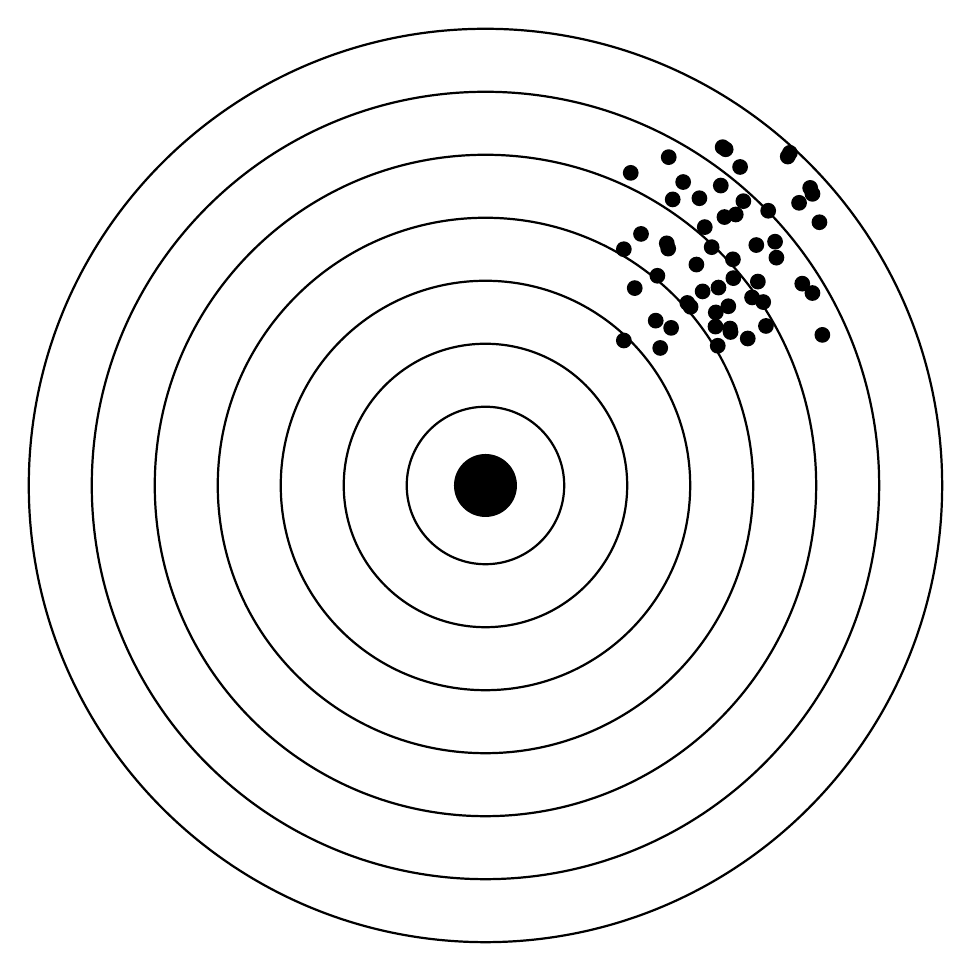
\begin{tikzpicture}
\def\farbea{black}
\def\farbeb{white}
\def\farbefill{\fuellung}
% mit verschiedenen ringen
%\foreach \x/\y in {  6/\farbea, 5/\farbeb, 4/\farbea, 3/\farbeb, 2/\farbea, 1/\farbeb} 
%{\draw[thick, fill=none, draw=black] (0,0) circle (\x cm);}

\foreach \x in { 1,1.8,...,6} 
{\draw[thick, fill=none, draw=black] (0,0) circle (\x cm);}

\draw[thick, fill=black, draw=none] (0,0) circle (.4 cm);

%oben rechts, reliable
 \def\shiftx{3}
 \def\shifty{3}
 \pgfmathsetseed{24122015}
 \foreach \p in {1,...,55}
 { \fill [\farbefill](1.3*rand+\shiftx,1.3*rand+\shifty) circle (0.1);
 }


%überall zerstreut
% \def\shiftx{0}
% \def\shifty{0}
% \pgfmathsetseed{24122015}
% \foreach \p in {1,...,55}
% { \fill [\farbefill](4.2*rand+\shiftx,4.2*rand+\shifty) circle (0.1);
% }


% %oberhalb zerstreut
% \def\shiftx{0}
% \def\shifty{2.5}
% \pgfmathsetseed{24122015}
% \foreach \p in {1,...,55}
% { \fill [\farbefill](3.4*rand+\shiftx,2.7*rand+\shifty) circle (0.1);
% }

%mittig alle
%\def\shiftx{0}
%\def\shifty{0}
%\pgfmathsetseed{24122015}
%\foreach \p in {1,...,55}
%{ \fill [\farbefill](1*rand+\shiftx,1*rand+\shifty) circle (0.1);
%}


\end{tikzpicture}

}
\end{tabular}
\subcaption{Hohe Reliabilität, Geringe Validität}
\end{subtable}
\hfill
\begin{subtable}[t]{0.22\linewidth}
\begin{tabular}{c}
\resizebox{.8\linewidth}{!}{%
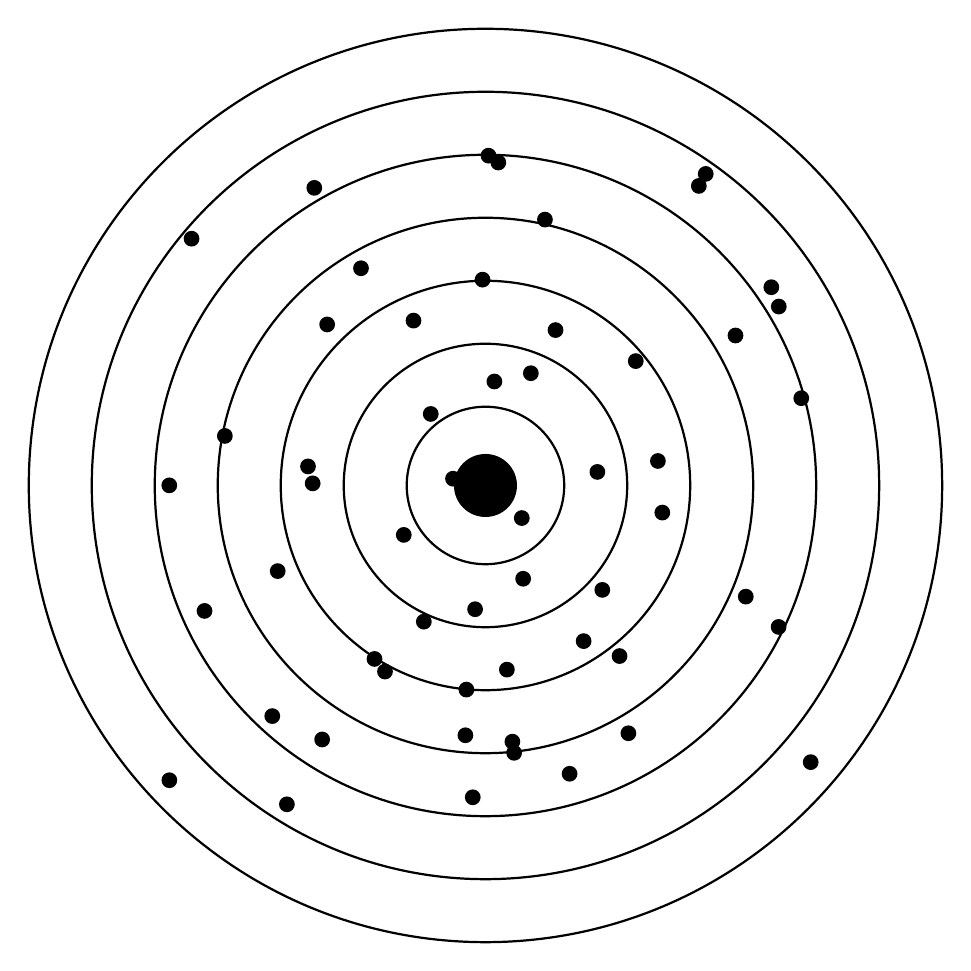
\begin{tikzpicture}
\def\farbea{black}
\def\farbeb{white}
\def\farbefill{\fuellung}
% mit verschiedenen ringen
%\foreach \x/\y in {  6/\farbea, 5/\farbeb, 4/\farbea, 3/\farbeb, 2/\farbea, 1/\farbeb} 
%{\draw[thick, fill=none, draw=black] (0,0) circle (\x cm);}

\foreach \x in { 1,1.8,...,6} 
{\draw[thick, fill=none, draw=black] (0,0) circle (\x cm);}

\draw[thick, fill=black, draw=none] (0,0) circle (.4 cm);

%oben rechts, reliable
% \def\shiftx{3}
% \def\shifty{3}
% \pgfmathsetseed{24122015}
% \foreach \p in {1,...,55}
% { \fill [\farbefill](1.3*rand+\shiftx,1.3*rand+\shifty) circle (0.1);
% }


%überall zerstreut
 \def\shiftx{0}
 \def\shifty{0}
 \pgfmathsetseed{24122015}
 \foreach \p in {1,...,55}
 { \fill [\farbefill](4.2*rand+\shiftx,4.2*rand+\shifty) circle (0.1);
 }


% %oberhalb zerstreut
% \def\shiftx{0}
% \def\shifty{2.5}
% \pgfmathsetseed{24122015}
% \foreach \p in {1,...,55}
% { \fill [\farbefill](3.4*rand+\shiftx,2.7*rand+\shifty) circle (0.1);
% }

%mittig alle
%\def\shiftx{0}
%\def\shifty{0}
%\pgfmathsetseed{24122015}
%\foreach \p in {1,...,55}
%{ \fill [\farbefill](1*rand+\shiftx,1*rand+\shifty) circle (0.1);
%}


\end{tikzpicture}

}
\end{tabular}
\subcaption{Geringe Reliabilität, Mittlere Validität}
\end{subtable}
\hfill
\begin{subtable}[t]{0.22\linewidth}
\begin{tabular}{c}
\resizebox{.8\linewidth}{!}{%
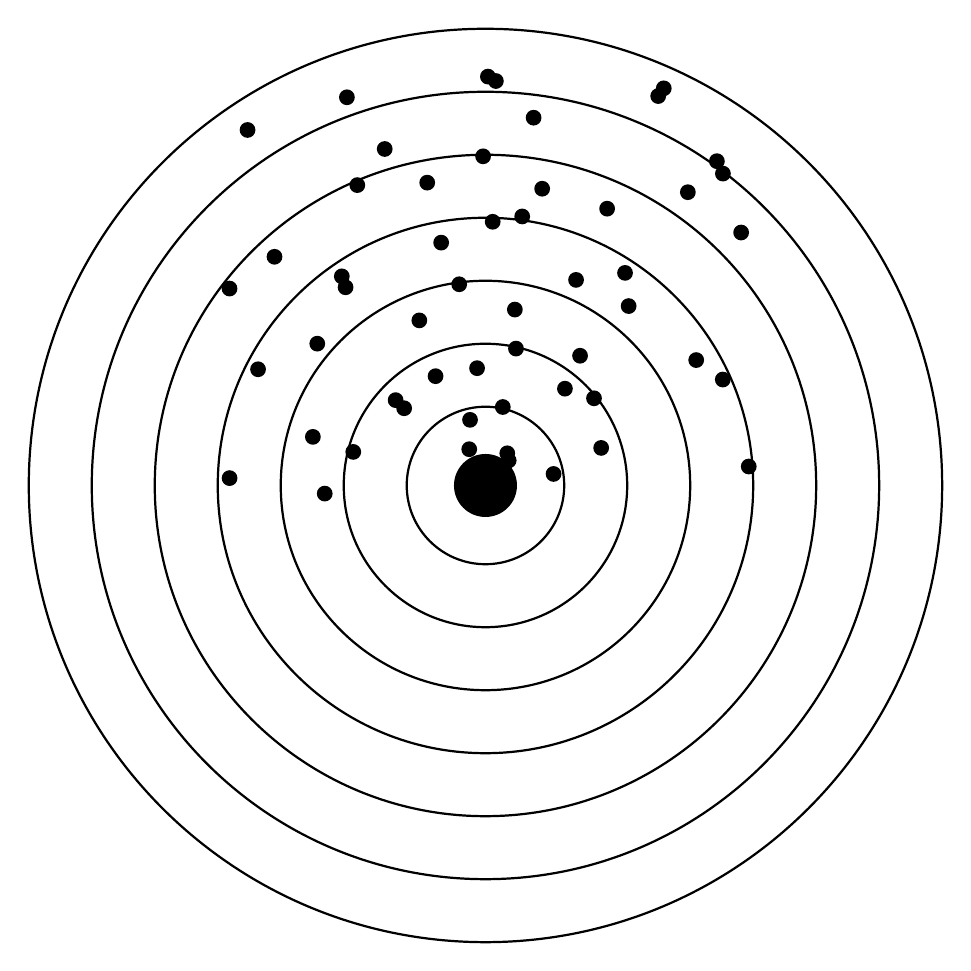
\begin{tikzpicture}
\def\farbea{black}
\def\farbeb{white}
\def\farbefill{\fuellung}
% mit verschiedenen ringen
%\foreach \x/\y in {  6/\farbea, 5/\farbeb, 4/\farbea, 3/\farbeb, 2/\farbea, 1/\farbeb} 
%{\draw[thick, fill=none, draw=black] (0,0) circle (\x cm);}

\foreach \x in { 1,1.8,...,6} 
{\draw[thick, fill=none, draw=black] (0,0) circle (\x cm);}

\draw[thick, fill=black, draw=none] (0,0) circle (.4 cm);

%oben rechts, reliable
% \def\shiftx{3}
% \def\shifty{3}
% \pgfmathsetseed{24122015}
% \foreach \p in {1,...,55}
% { \fill [\farbefill](1.3*rand+\shiftx,1.3*rand+\shifty) circle (0.1);
% }


%überall zerstreut
% \def\shiftx{0}
% \def\shifty{0}
% \pgfmathsetseed{24122015}
% \foreach \p in {1,...,55}
% { \fill [\farbefill](4.2*rand+\shiftx,4.2*rand+\shifty) circle (0.1);
% }


% %oberhalb zerstreut
 \def\shiftx{0}
 \def\shifty{2.5}
 \pgfmathsetseed{24122015}
 \foreach \p in {1,...,55}
 { \fill [\farbefill](3.4*rand+\shiftx,2.7*rand+\shifty) circle (0.1);
 }

%mittig alle
%\def\shiftx{0}
%\def\shifty{0}
%\pgfmathsetseed{24122015}
%\foreach \p in {1,...,55}
%{ \fill [\farbefill](1*rand+\shiftx,1*rand+\shifty) circle (0.1);
%}


\end{tikzpicture}

}
\end{tabular}
\subcaption{Geringe Reliabilität, Geringe Validität}
\end{subtable}
\hfill
\begin{subtable}[t]{0.22\linewidth}
\begin{tabular}{c}
\resizebox{.8\linewidth}{!}{%
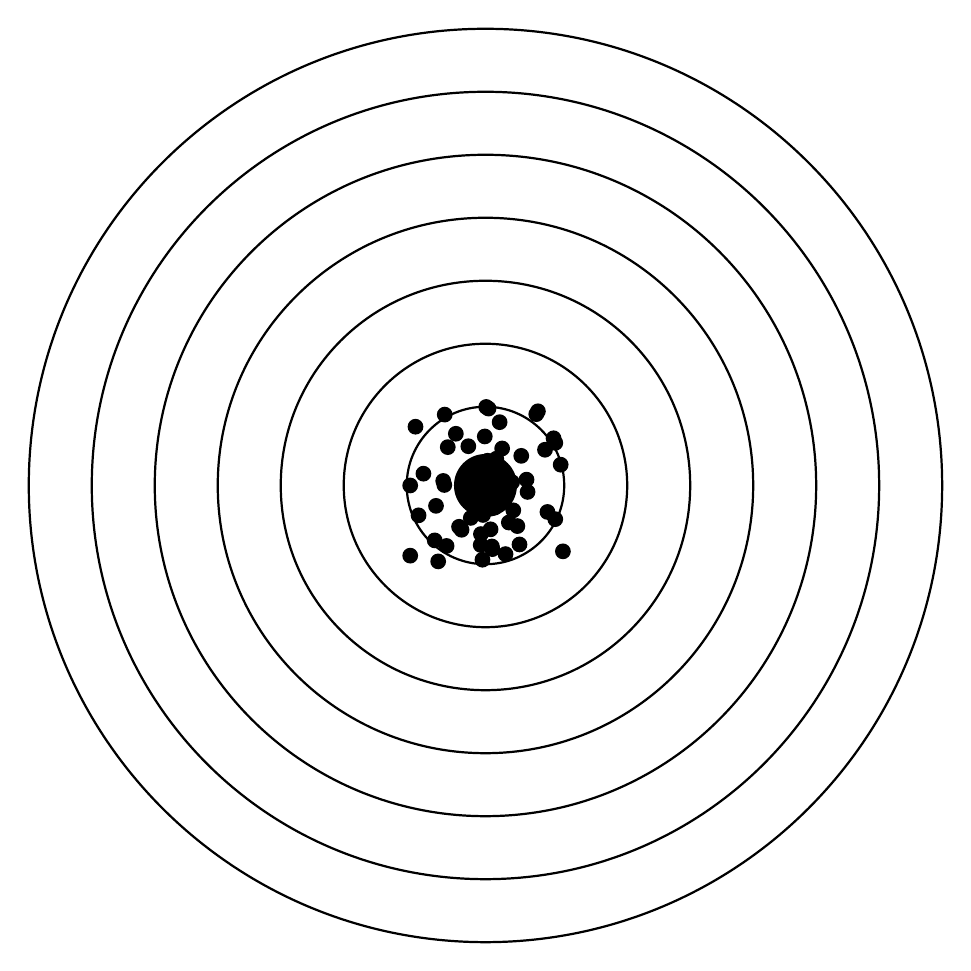
\begin{tikzpicture}
\def\farbea{black}
\def\farbeb{white}
\def\farbefill{\fuellung}
% mit verschiedenen ringen
%\foreach \x/\y in {  6/\farbea, 5/\farbeb, 4/\farbea, 3/\farbeb, 2/\farbea, 1/\farbeb} 
%{\draw[thick, fill=none, draw=black] (0,0) circle (\x cm);}

\foreach \x in { 1,1.8,...,6} 
{\draw[thick, fill=none, draw=black] (0,0) circle (\x cm);}

\draw[thick, fill=black, draw=none] (0,0) circle (.4 cm);

%oben rechts, reliable
% \def\shiftx{3}
% \def\shifty{3}
% \pgfmathsetseed{24122015}
% \foreach \p in {1,...,55}
% { \fill [\farbefill](1.3*rand+\shiftx,1.3*rand+\shifty) circle (0.1);
% }


%überall zerstreut
% \def\shiftx{0}
% \def\shifty{0}
% \pgfmathsetseed{24122015}
% \foreach \p in {1,...,55}
% { \fill [\farbefill](4.2*rand+\shiftx,4.2*rand+\shifty) circle (0.1);
% }


% %oberhalb zerstreut
% \def\shiftx{0}
% \def\shifty{2.5}
% \pgfmathsetseed{24122015}
% \foreach \p in {1,...,55}
% { \fill [\farbefill](3.4*rand+\shiftx,2.7*rand+\shifty) circle (0.1);
% }

%mittig alle
\def\shiftx{0}
\def\shifty{0}
\pgfmathsetseed{24122015}
\foreach \p in {1,...,55}
{ \fill [\farbefill](1*rand+\shiftx,1*rand+\shifty) circle (0.1);
}


\end{tikzpicture}

}
\end{tabular}
\subcaption{Hohe Reliabilität, Hohe Validität}
\end{subtable}

\caption{ Fachgebiet und Logo}
\end{table}


\begin{table}[H]
\centering
\caption{My Caption}
\label{tab: myLabel}
\resizebox{\textwidth}{!}{%
\begin{tabular}{C{.25\textwidth}C{.25\textwidth}C{.25\textwidth}C{.25\textwidth}}
\resizebox{.82\linewidth}{!}{%
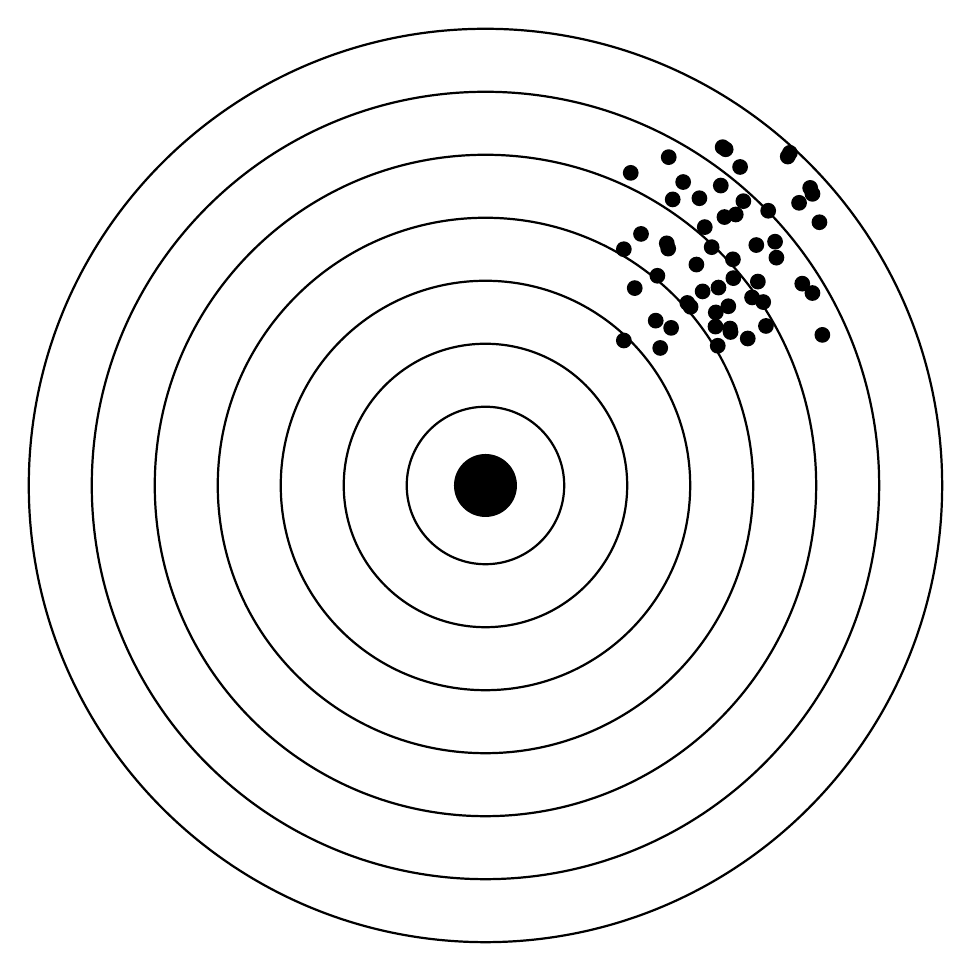
\begin{tikzpicture}
\def\farbea{black}
\def\farbeb{white}
\def\farbefill{\fuellung}
% mit verschiedenen ringen
%\foreach \x/\y in {  6/\farbea, 5/\farbeb, 4/\farbea, 3/\farbeb, 2/\farbea, 1/\farbeb} 
%{\draw[thick, fill=none, draw=black] (0,0) circle (\x cm);}

\foreach \x in { 1,1.8,...,6} 
{\draw[thick, fill=none, draw=black] (0,0) circle (\x cm);}

\draw[thick, fill=black, draw=none] (0,0) circle (.4 cm);

%oben rechts, reliable
 \def\shiftx{3}
 \def\shifty{3}
 \pgfmathsetseed{24122015}
 \foreach \p in {1,...,55}
 { \fill [\farbefill](1.3*rand+\shiftx,1.3*rand+\shifty) circle (0.1);
 }


%überall zerstreut
% \def\shiftx{0}
% \def\shifty{0}
% \pgfmathsetseed{24122015}
% \foreach \p in {1,...,55}
% { \fill [\farbefill](4.2*rand+\shiftx,4.2*rand+\shifty) circle (0.1);
% }


% %oberhalb zerstreut
% \def\shiftx{0}
% \def\shifty{2.5}
% \pgfmathsetseed{24122015}
% \foreach \p in {1,...,55}
% { \fill [\farbefill](3.4*rand+\shiftx,2.7*rand+\shifty) circle (0.1);
% }

%mittig alle
%\def\shiftx{0}
%\def\shifty{0}
%\pgfmathsetseed{24122015}
%\foreach \p in {1,...,55}
%{ \fill [\farbefill](1*rand+\shiftx,1*rand+\shifty) circle (0.1);
%}


\end{tikzpicture}

}  & \resizebox{.8\linewidth}{!}{%
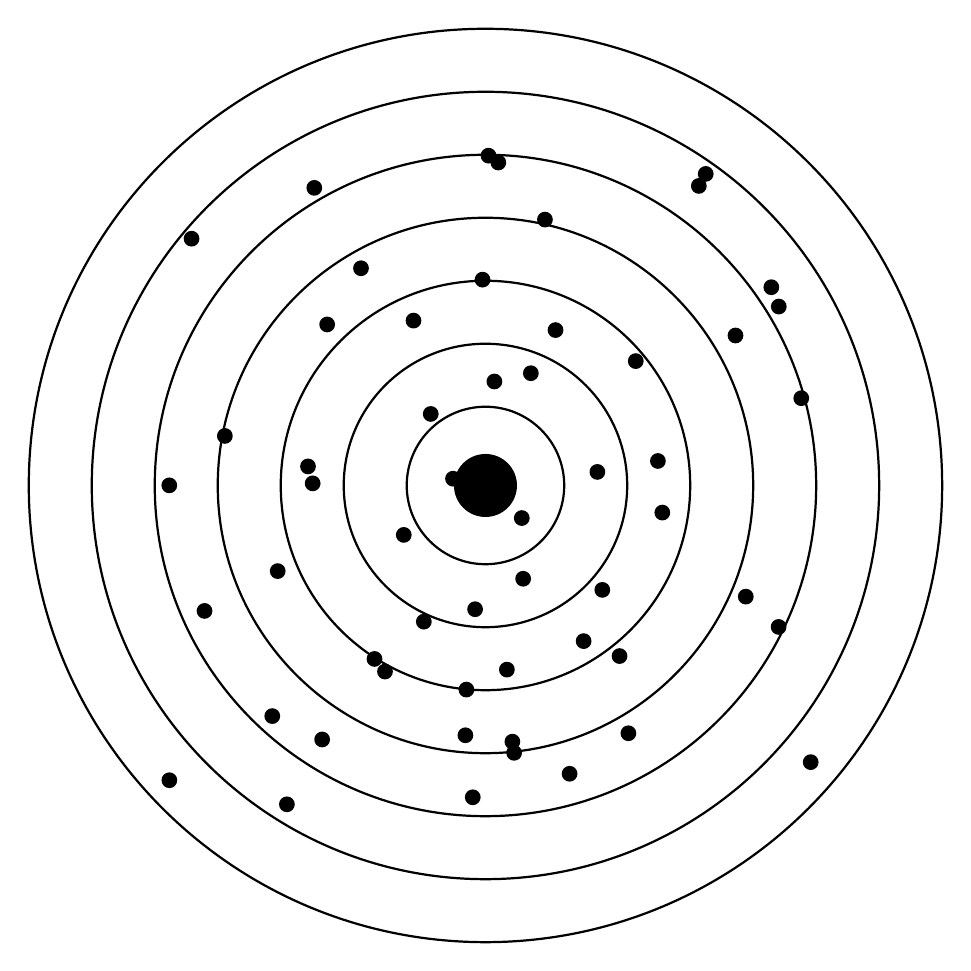
\begin{tikzpicture}
\def\farbea{black}
\def\farbeb{white}
\def\farbefill{\fuellung}
% mit verschiedenen ringen
%\foreach \x/\y in {  6/\farbea, 5/\farbeb, 4/\farbea, 3/\farbeb, 2/\farbea, 1/\farbeb} 
%{\draw[thick, fill=none, draw=black] (0,0) circle (\x cm);}

\foreach \x in { 1,1.8,...,6} 
{\draw[thick, fill=none, draw=black] (0,0) circle (\x cm);}

\draw[thick, fill=black, draw=none] (0,0) circle (.4 cm);

%oben rechts, reliable
% \def\shiftx{3}
% \def\shifty{3}
% \pgfmathsetseed{24122015}
% \foreach \p in {1,...,55}
% { \fill [\farbefill](1.3*rand+\shiftx,1.3*rand+\shifty) circle (0.1);
% }


%überall zerstreut
 \def\shiftx{0}
 \def\shifty{0}
 \pgfmathsetseed{24122015}
 \foreach \p in {1,...,55}
 { \fill [\farbefill](4.2*rand+\shiftx,4.2*rand+\shifty) circle (0.1);
 }


% %oberhalb zerstreut
% \def\shiftx{0}
% \def\shifty{2.5}
% \pgfmathsetseed{24122015}
% \foreach \p in {1,...,55}
% { \fill [\farbefill](3.4*rand+\shiftx,2.7*rand+\shifty) circle (0.1);
% }

%mittig alle
%\def\shiftx{0}
%\def\shifty{0}
%\pgfmathsetseed{24122015}
%\foreach \p in {1,...,55}
%{ \fill [\farbefill](1*rand+\shiftx,1*rand+\shifty) circle (0.1);
%}


\end{tikzpicture}

}      & \resizebox{.8\linewidth}{!}{%
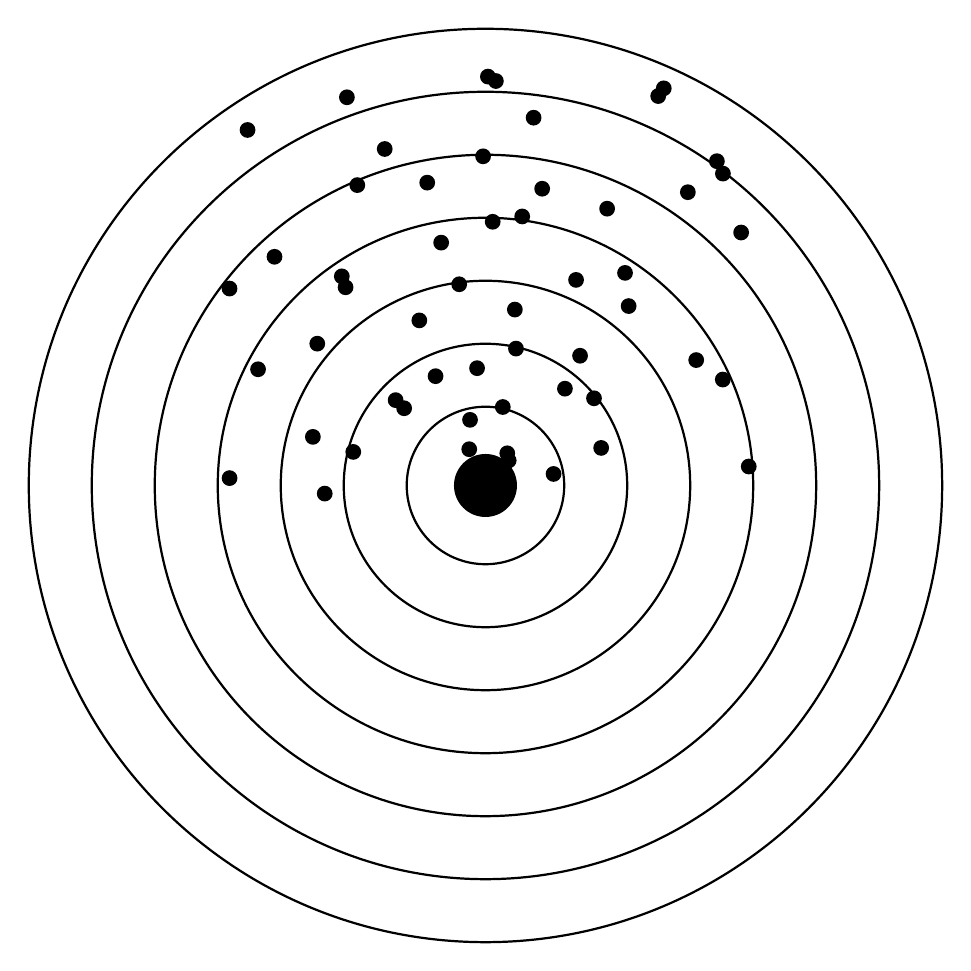
\begin{tikzpicture}
\def\farbea{black}
\def\farbeb{white}
\def\farbefill{\fuellung}
% mit verschiedenen ringen
%\foreach \x/\y in {  6/\farbea, 5/\farbeb, 4/\farbea, 3/\farbeb, 2/\farbea, 1/\farbeb} 
%{\draw[thick, fill=none, draw=black] (0,0) circle (\x cm);}

\foreach \x in { 1,1.8,...,6} 
{\draw[thick, fill=none, draw=black] (0,0) circle (\x cm);}

\draw[thick, fill=black, draw=none] (0,0) circle (.4 cm);

%oben rechts, reliable
% \def\shiftx{3}
% \def\shifty{3}
% \pgfmathsetseed{24122015}
% \foreach \p in {1,...,55}
% { \fill [\farbefill](1.3*rand+\shiftx,1.3*rand+\shifty) circle (0.1);
% }


%überall zerstreut
% \def\shiftx{0}
% \def\shifty{0}
% \pgfmathsetseed{24122015}
% \foreach \p in {1,...,55}
% { \fill [\farbefill](4.2*rand+\shiftx,4.2*rand+\shifty) circle (0.1);
% }


% %oberhalb zerstreut
 \def\shiftx{0}
 \def\shifty{2.5}
 \pgfmathsetseed{24122015}
 \foreach \p in {1,...,55}
 { \fill [\farbefill](3.4*rand+\shiftx,2.7*rand+\shifty) circle (0.1);
 }

%mittig alle
%\def\shiftx{0}
%\def\shifty{0}
%\pgfmathsetseed{24122015}
%\foreach \p in {1,...,55}
%{ \fill [\farbefill](1*rand+\shiftx,1*rand+\shifty) circle (0.1);
%}


\end{tikzpicture}

} & \resizebox{.8\linewidth}{!}{%
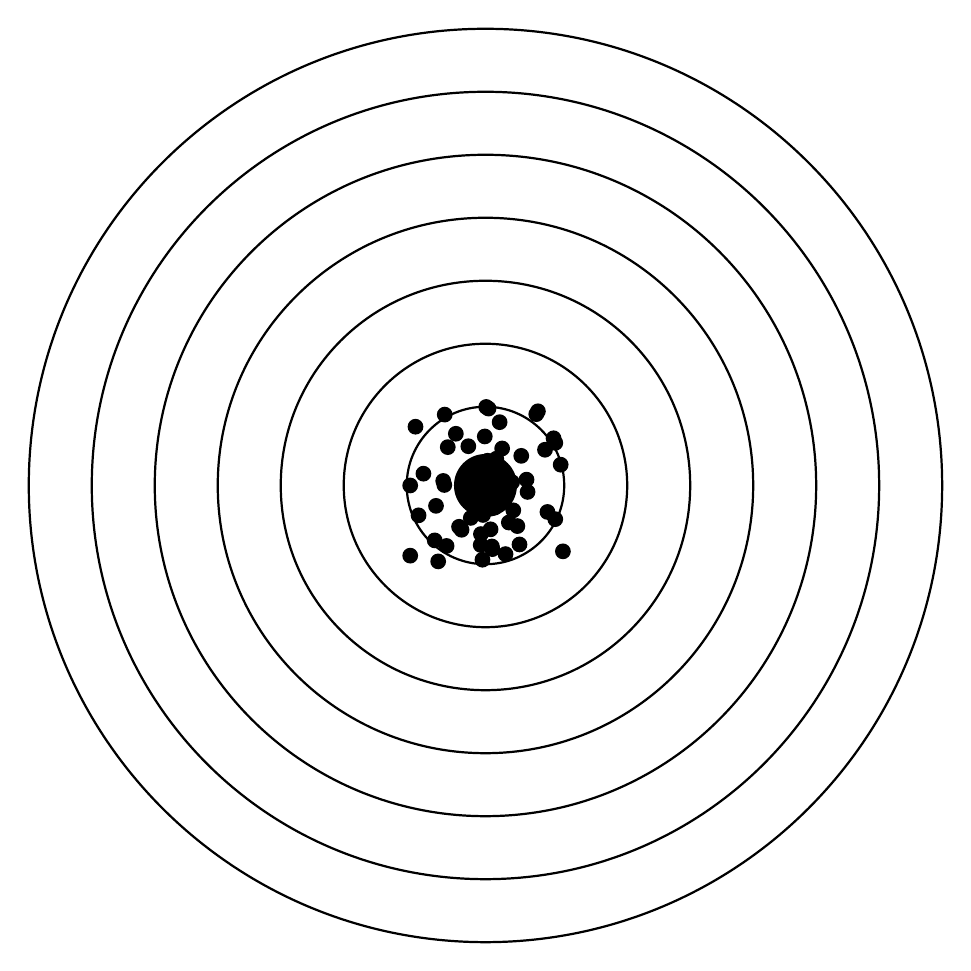
\begin{tikzpicture}
\def\farbea{black}
\def\farbeb{white}
\def\farbefill{\fuellung}
% mit verschiedenen ringen
%\foreach \x/\y in {  6/\farbea, 5/\farbeb, 4/\farbea, 3/\farbeb, 2/\farbea, 1/\farbeb} 
%{\draw[thick, fill=none, draw=black] (0,0) circle (\x cm);}

\foreach \x in { 1,1.8,...,6} 
{\draw[thick, fill=none, draw=black] (0,0) circle (\x cm);}

\draw[thick, fill=black, draw=none] (0,0) circle (.4 cm);

%oben rechts, reliable
% \def\shiftx{3}
% \def\shifty{3}
% \pgfmathsetseed{24122015}
% \foreach \p in {1,...,55}
% { \fill [\farbefill](1.3*rand+\shiftx,1.3*rand+\shifty) circle (0.1);
% }


%überall zerstreut
% \def\shiftx{0}
% \def\shifty{0}
% \pgfmathsetseed{24122015}
% \foreach \p in {1,...,55}
% { \fill [\farbefill](4.2*rand+\shiftx,4.2*rand+\shifty) circle (0.1);
% }


% %oberhalb zerstreut
% \def\shiftx{0}
% \def\shifty{2.5}
% \pgfmathsetseed{24122015}
% \foreach \p in {1,...,55}
% { \fill [\farbefill](3.4*rand+\shiftx,2.7*rand+\shifty) circle (0.1);
% }

%mittig alle
\def\shiftx{0}
\def\shifty{0}
\pgfmathsetseed{24122015}
\foreach \p in {1,...,55}
{ \fill [\farbefill](1*rand+\shiftx,1*rand+\shifty) circle (0.1);
}


\end{tikzpicture}

} \\
&&&\\
	(a) Hohe Reliabilität, Geringe Validität 1& (b) Geringe Reliabilität, Mittlere Validität& (c) Geringe Reliabilität, Geringe Validität & (d) Hohe Reliabilität, Hohe Validität\\
\end{tabular}}
\end{table}



\begin{figure} [H]
\centering
\resizebox{.3\textwidth}{!}{%
\begin{tikzpicture}[every node/.style={anchor=center},>=stealth']
\matrix (m) [matrix of math nodes, row sep=3em, column sep=3em, ampersand replacement=\&]
{ A \& B \\
  C \& D \\ 
  \& \&E\\};
\draw[->] (m-1-1) -- node[above] {$\scriptstyle f$} (m-1-2);
\draw[->] (m-1-2) -- node[right] {$\scriptstyle j$} (m-2-2);
\draw[->] (m-1-1) -- node[left]  {$\scriptstyle i$} (m-2-1);
\draw[->] (m-2-1) -- node[below] {$\scriptstyle g$} (m-2-2);
\draw[->] (m-2-1) -- node[below] {$\scriptstyle g$} (m-3-3);
\draw[->] (m-1-2) -- node[below] {$\scriptstyle g$} (m-3-3);
\end{tikzpicture}}
\caption{Caption}
\label{fig:my_label}
\end{figure}






\begin{tikzcd}
r \arrow[rr, bend left] & z & t \arrow[dd] \\
 & x \arrow[rd] \arrow[u] &  \\
y \arrow[ru] \arrow[uu] &  & z \arrow[ll]
\end{tikzcd}

\resizebox{1\linewidth}{!}{% standard .82
\begin{tikzpicture}[every node/.style={anchor=center},>=stealth]
     \matrix (tree) [%
       matrix of nodes,
       minimum size=1cm,
       column sep=1cm,
       row sep=.5cm,
       ampersand replacement=\&,
       row 1/.style={nodes={draw,top color=white, bottom color=black!20,rounded corners, text width=2cm, align=center, outer sep=.1cm}},
       row 3/.style={nodes={draw,top color=white, bottom color=black!20,rounded corners, text width=2cm, align=center, outer sep=.1cm}},
       ]
     {
         \& {Domäne \\ } \& \\
         \&\quad\&\\
     Field  \& \&  Person\\
     };

%      \draw[->] (tree-1-2) -- (tree-3-1) node [midway,above] {$p$};
%      \draw[->] (tree-1-2) -- (tree-3-3) node [midway,below] {$1-p$};
%     \draw[] (tree-3-1) -- (tree-3-3) node [midway,below] {$1-p$};
%      \draw[->] (tree-3-3) -- (tree-3-1) node [midway,below] {$1-p$};
\draw (tree-1-2) to [bend left=0] node [above, fill=none, sloped] {informiert} (tree-3-3)  ;
\draw (tree-1-2) to [bend left=0]  node [above, sloped] {übernimmt} (tree-3-1);
\draw (tree-3-1) to [bend left=5]  node [above] {überträgt} (tree-3-3);
\draw (tree-3-3) to [bend left=5]  node [below] {bewertet} (tree-3-1);

\end{tikzpicture}
}




